\documentclass[12]{article}

\usepackage{amsmath}
\usepackage{enumerate}
\usepackage{fancyhdr}
\usepackage{color}
\usepackage{listings}
\usepackage{graphicx}
\usepackage{amssymb}

\newcommand{\norm}[1]{\left\lVert#1\right\rVert}
\DeclareMathOperator*{\argmin}{arg\,min}

\definecolor{lightgray}{gray}{0.5}

\begin{document}

\title{Stochastic Optimization for Strategy Selection}
\author{Ryan McKenna}
\date{\today}
\maketitle

\section{Motivation}

We showed that it is tractable to solve the matrix mechanism optimization problem for arbitrary workloads if $ n \leq 8192 $ and for workloads made from kronecker building blocks if the strategy is restricted to either be a (single) kronecker product or a set of weighted marginals.  The key that made these restricted optimization problems tractable to solve was that the pseudo inverse of the strategy had an exploitable structure.

In particular, the pseudo inverse of $(A^T A)$ is a kroneccker product when $A$ is a kronecker product, and is a sum of kronecker products when $A$ is weighted marginals.  This structure was enough to efficiently evaluate the objective/gradient and solve the optimization problem.  It would have been nice if we could directly optimize over a strategy that is a union of kronecker products, but unfortunately we had to resort to heuristic methods.

It would also be nice if we could optimize over a large sparse strategy (with fixed sparsity structure).  For example, if we wanted to find a strategy for AllRange(16384) we couldn't do that using already developed techniques.  While it's certainly possible to find a pretty good strategy by extrapolating the strategy for AllRange(8192), it would be nice to have a more principled way to do it.  

\section{Problem Statement}

Given a strategy parameterization with a compact representation (e.g., sparse or kronecker product based) such that $Av$ and $A^T v$ can be computed efficiently, solve the matrix mechanism optimization problem.  

We assume that some structure has been imposed on the strategy.  It's impossible to optimize over all possible strategies $A$ when $n$ is large because even representing an arbitrary strategy takes too much memory, let alone optimizing it.  

\subsection{Sparse Strategies}

We might want to restrict the optimization to strategies that have a fixed sparsity structure.  For example, if we wanted to optimize AllRange(128), we could impose the following sparsity structure:

\begin{center}
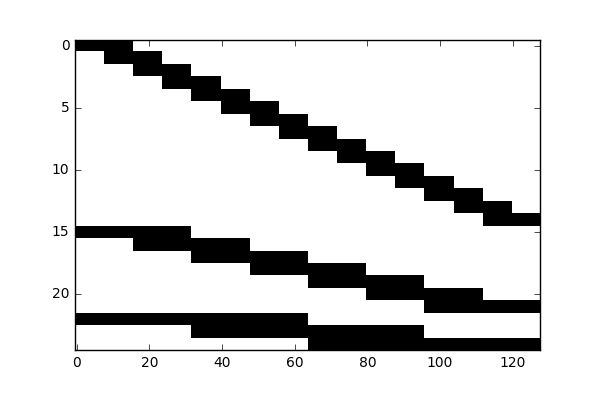
\includegraphics[width=0.5\textwidth]{sparse_structure} 
\end{center}

the above plot can be interpreted as a matrix, where a white cell is a structural zero, and a black cell is a  free parameter (to be optimized over).  Identity queries are also present in the above strategy, but not shown.  We know that the optimal strategy looks something like this, so it is a reasonable structure to impose.  While imposing this type of structure may make it impossible to find the best strategy, it does make it easier to find good strategies (assuming the imposed structure is good). 
Using this type of structure on the strategy for AllRange(8192) results in 30x fewer free parameters to optimize over than if no sparsity structure was assumed.

\subsection{Union of Kron Strategies}

For the workload $ \begin{bmatrix} R \otimes T \\ T \otimes R \end{bmatrix} $ we expect the optimal strategy to be of the form $ \begin{bmatrix} B \otimes T \\ T \otimes B \end{bmatrix} $.  The techniques we've developed so far to handle these types of cases is heuristic in nature and leaves something to be desired.  For this simple case, letting $B$ be the optimal strategy for $R$ will be near optimal.  For more complicated workloads, it won't always be clear what the optimal strategy will look like, but we'd like to be able to impose this type of structure on it to find it with limited domain expertise.  For example, maybe we'd just like to optimize over a union of 2 arbitrary kronecker products:

$$ \begin{bmatrix} A^{(1)}_1 \otimes A^{(1)}_2 \\ A^{(2)}_1 \otimes A^{(2)}_2 \end{bmatrix} $$

Of course, the more structure that is imposed, the more efficient the optimization will be.  But it is nice to be able to optimize over strategies in the above form because of their generality.  

\section{Technical Details}

Given a strategy $A \in \mathbb{R}^{p \times n}$ and a workload $ W \in \mathbb{R}^{m \times n} $ we would like to compute the expected error of $A$ on $W$.  However, we assume it is intractable to do this directly, but that it is possible to get an stochastic estimate of the error (i.e., we assume solving a least squares problem with $A$ is fast).  The error of $A$ on $W$ can be written as:

$$ Error(W, A) = \mathbb{E}[|| W A^+ y ||_2^2] $$

where the expectation is taken with respect to the random $p \times 1 $ vector $y$ (sampled from a laplace distribution).  To get a stochastic estimate of the error, we can (1) sample $y$ from laplace distribution, (2) solve the least squares problem $z = A^+ y$, and (3) compute $ || W z ||_2^2 $.

For fixed $W$ and $y$, the estimated error can be written as 

$$ C(A) = || W A^+ y ||_2^2 = (A^+ y)^T (W^T W) (A^+ y) $$

It is fairly clear that we can evaluate $C(A)$ efficiently assuming we can solve the least squares problem $z = A^+ y$ and $W^T W$ has a representation that allows us to compute $(W^T W) z$ efficiently (e.g., if $W$ is a union of kronecker products, or is sparse, or only has a small number of queries).  But can we evaluate the gradient efficiently too?

\subsection{Gradient Derivations}

We first write $C(A)$ as the composition of several ``primitive'' functions:

\begin{align*}
C(A) &= f(z(B(A))) \\
f(z) &= z^T (W^T W) z \\
z(B) &= B y \\
B(A) &= A^+ \\
\end{align*}

We can work out the desired gradient $ \frac{\partial C}{\partial A} $ by working out the gradients and jacobians of the primitive functions, and applying the multivariate chain rule.

The first gradient is simple to express in vector form: 

$$ \frac{\partial f}{\partial z} = 2 (W^T W) z $$

The elementwise derivative of $z(B)$ is given by:

\begin{align*}
\frac{\partial z_i}{\partial B_{ij}} = y_j \\
\frac{\partial z_k}{\partial B_{ij}} = 0  & \:\:\:\: i \neq k \\
\end{align*}

it's difficult to reason about these derivatives in matrix form because it requries $3$ indices to characterize a single partial derivative.  However, by using the multivariate chain rule, we can work out the derviative of $f(z(B)) $ with respect to $B$.

\begin{align*}
\frac{\partial (f \circ z)}{\partial B_{ij}} &= \sum_k \frac{\partial f}{\partial z_k} \frac{\partial z_k}{\partial B_{ij}} \\
&= \frac{\partial f}{\partial z_i} y_j 
\end{align*}

In matrix form, this can be written as:

$$ \frac{\partial (f \circ z)}{B} = outer\Big(\frac{\partial f}{\partial z}, y\Big) = \Big( \frac{\partial f}{\partial z} \Big) y^T $$

Now we have to work out the partial derivatives of $ f(z(B(A))) $ with respect to $A$.  Let $\partial B$ be shorthand notation for $ \frac{\partial (f \circ z)}{\partial B} $.  Then:

$$ \frac{\partial (f \circ z \circ B)}{\partial A} = -A^+ (\partial B)^T A^+ + A^+ A^{+T} (\partial B) (I_p - A A^+) + (I_n - A^+ A) (\partial B) A^{+T} A^+ $$

Calculating this partial derivative matrix directly would be intractable.  However, since $ \partial B $ is an outer product, and matrix-multiplication is associative, we don't have to evaluate this expression directly.  Using $ \partial z = \frac{\partial f}{\partial z} $ as shorthand notation, we can express $ \frac{\partial C}{\partial A} $ as:

$$ \frac{\partial C}{\partial A} = -[A^+ y] [(\partial z)^T A^+] + [A^+ A^{+T} (\partial z)] [y^T (I_p - A A^+)] + [(I_n - A^+ A) (\partial z)] [y^T A^{+T} A^+] $$

Note that this expression only requires solving at most $8$ instances of least squares (one for each pseudo inverse).  However, because some of the least squares problems are identitical, we only need to solve $5$ unique instances (in addition to the $1$ required to calculate the objective function).  If $A$ has full column rank (e.g., if it is a p-Identity strategy), then the third term becomes $0$ and can be dropped.  Similarly if $A$ has full row rank, then the second term can be dropped.

From the equation above, one can see that the gradient $ \frac{\partial C}{\partial A} $ is the sum of $3$ outer products and thus has a compact representation that we can exploit (i.e., it is a rank $3$ matrix).  Due to this compact representation of the gradient we can use this technique for $A$ matrices that are too large to fit into memory as a dense matrix.

However, note that $ \frac{\partial C}{\partial A}$ is not exactly what we are looking for: we assume $A$ has been parameterized by a set of variables so that $ A = A(\theta) $.  We need to calculate $ \frac{\partial (C \circ A)}{\partial \theta} $ \emph{without the explicit representation of $ \frac{\partial C}{\partial A} $}.   In the following sections, we outline the main ideas of how to do this if $A$ has a sparsity structure or if $A$ is a union of kron products.  

\subsection{Parameterized Gradient}

We showed how to calculate the gradient of the objective function with respect to $A$, but now we want to calculate the gradient with respect to $\theta$ where $ A = A(\theta) $ while respecting the compact representation of $\frac{\partial C}{\partial A}$ and not materializing the full matrix (which is assumed to be too large to fit into memory). 

\textbf{Sparsity Structure}

If $A$ has a fixed sparsity structure with up to $K$ nonzero entries, then it can be parameterized by a length $K$ vector $\theta$, so that the $k^{th}$ nonzero entry of $A$ (located at index $r_k, c_k$) has value $\theta_k$.  The gradient of the objective function with respect to $\theta_k$ is given below:

$$ \frac{\partial (C \circ A)}{\partial \theta_k} = \Big(\frac{\partial C}{\partial A}\Big)_{r_k, c_k} $$

We can calculate this gradient in $O(K)$ time using the compact representation of the gradient with respect to $A$ (as opposed to $O(p n)$ time if the full matrix had to be materialized).  The $O(K)$ method directly calculates the entries of the gradient matrix that it needs, without calculating the entries that it doesn't need.


\textbf{Kronecker Product}

If $A = B \otimes C $ is a kronecker product, then it can be parameterized by $ \theta = (B,C) $.  If $B$ is $m_1 \times n_1$ and $C$ is $m_2 \times n_2$, then the gradient with respect to $A$ can be written as the sum of 3 outer products.  Assume for simplicity that it can be written as a single outer product (which occurs if $A$ is square and invertible).

$$ \frac{\partial C}{\partial A} = u v^T $$ 

where $u$ and $v$ are length $m_1 m_2$ and $n_1 n_2$ column vectors.  We'd like to recover $ \frac{\partial (C \circ A)}{\partial B} $ without materializing the $m_1 m_2 \times n_1 n_2 $ outer product matrix.  If $u$ and $v$ are reorganized into $m_1 \times m_2 $ and $n_1 \times n_2 $ matrices $U$ and $V$, so that the cell $ B_{ij} C_{kl} $ corresponds to $ U_{ik} V_{jl} $, then we can express the desired gradient as:

$$ \frac{\partial (C \circ A)}{\partial B_{ij}} = \sum_{kl} U_{ik} V_{jl} C_{kl} $$

In matrix form, this is equivalent to:

$$ \frac{\partial (C \circ A)}{\partial B} = U C V^T $$

The gradient with respect to $C$ is similar.  The techniques can be modified if $A$ is a kronecker product of more than 2 things, and it can also be modified if $A$ is a union of kronecker products.  

\subsection{Uniform Column Norm}

We showed how to calculate the gradient of the objective function $ || W A^+ y ||_F^2 $ but haven't accounted for the sensitivity of $A$ yet.  A projected gradient method could be applied, or a subgradient method could be used.  A better approach is to setup $A$ so that it always has uniform column norm.  One way to accomplish this is to take the input matrix, say $P$ and scale every entry by the sensitivity of the corresponding column, resulting in a strategy $A$ that has uniform column norm.  

$$ A_{ij} = \frac{P_{ij}}{\sum_{k} P_{kj}} $$

We know that 

$$ \frac{\partial (C \circ A)}{\partial P_{kj}} = \sum_{i} \frac{\partial C}{\partial A_{ij}} \frac{\partial A_{ij}}{\partial P_{kj}} $$

we assume we have access to $ \frac{\partial C}{\partial A_{ij}} $ -- recall that it is the sum of 3 outer products.  We can easily derive $ \frac{\partial A_{ij}}{\partial P_{kj}} $:

$$ \frac{\partial A_{ij}}{\partial P_{kj}} = 
\begin{cases}
\frac{\Sigma - P_{ij}}{\Sigma^2} & i = k \\
\frac{- P_{ij}}{\Sigma^2} & i \neq k \\
\end{cases} $$

where $ \Sigma $ is shorthand notation for $ \sum_k P_{kj} $.  Plugging into the equation from above, we get:

$$ \frac{\partial (C \circ A)}{\partial P_{kj}} = -\sum_{i} \frac{\partial C}{\partial A_{ij}} \frac{P_{ij}}{\Sigma^2} + \frac{\partial C}{\partial A_{kj}} \frac{1}{\Sigma} $$

If $D$ is the diagonal scaling matrix whose entries are $ 1/\Sigma_j $, and $1$ is the square matrix of ones, and $ \odot $ is the elementwise product, then the derivative can be expressed in matrix form as:

$$ \frac{\partial (C \circ A)}{\partial P} = -1 \Big(\frac{\partial C}{\partial A} \odot P \Big) D^2 + \frac{\partial C}{\partial A} D $$

We know that $ \frac{\partial C}{\partial A} $ has a compact representation as the sum of three outer products, and using the equation above it can be shown that $ \frac{\partial (C \circ A)}{\partial P} $ has a compact representation as the sum of four outer products.  Importantly, it can be obtained without inspecting the entries of $P$, only the matrix vector product $P^T u$ is necessary. 

\end{document}
